\documentclass[12pt,a4paper,notitlepage]{article}
\usepackage[utf8]{inputenc}
\usepackage[english]{babel}
\usepackage{mathtools}
\usepackage{titling}
\usepackage{amsfonts}
\usepackage{amssymb}
\usepackage{amsthm}
\usepackage{pgfplots}
\usepackage[caption = false]{subfig}
\usepackage{caption}
\usepackage{graphicx}
\usepackage{tikz-3dplot}
\usepackage{subcaption}
\usepackage{float}
\usepackage{adjustbox}
\usepackage{multirow,rotating}
\usepackage[autostyle]{csquotes}
\usepackage[toc,page]{appendix}
\DeclareUnicodeCharacter{20AC}{\euro}
\usepackage[backend=biber,
			style=authoryear-comp,
			isbn=false,
			doi=false,
			bibstyle=authoryear,
			natbib,
			]{biblatex}

\begin{document}

\section{Online News} 

\begin{figure}[H]\centering
\caption{Time Series of visits (subsample 1)}
	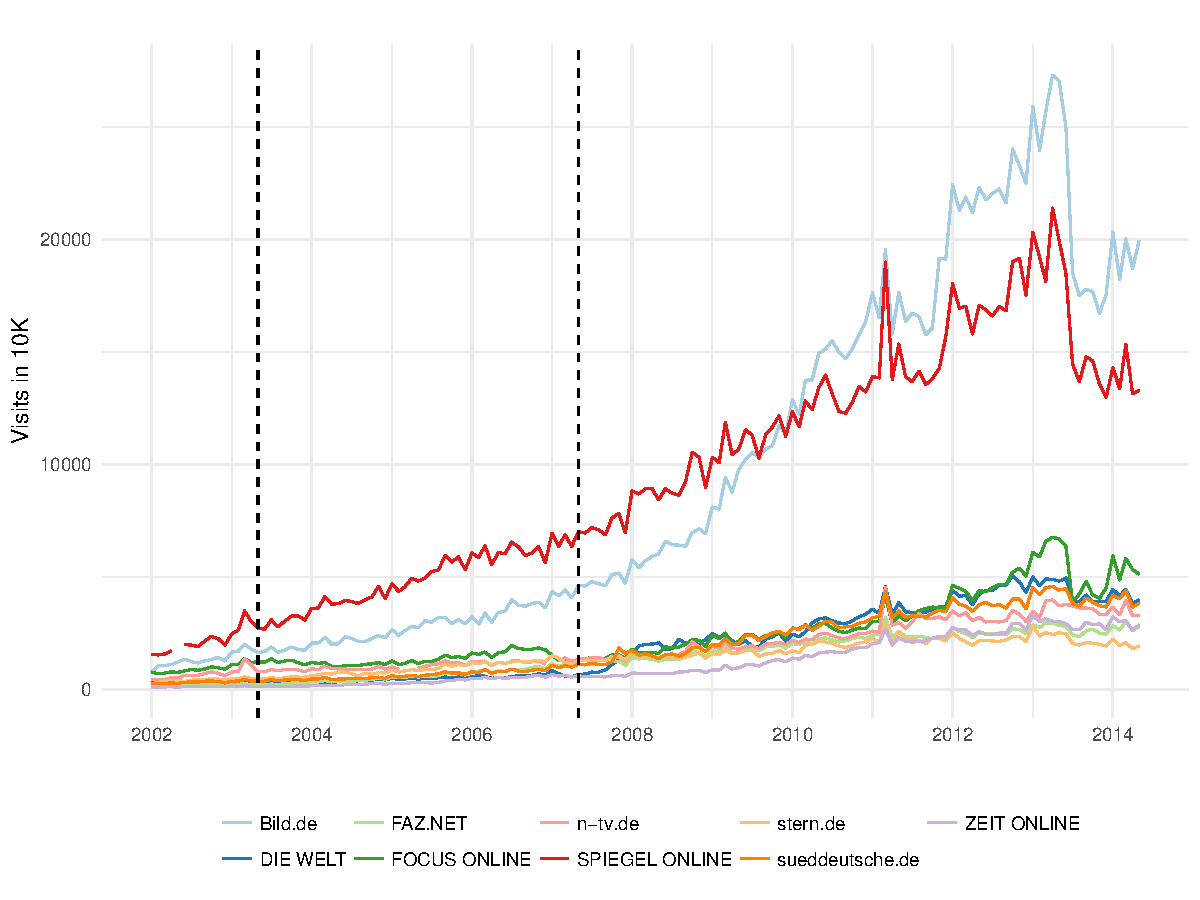
\includegraphics[scale=.6]{../figs/fig_news1}
	\label{}
\end{figure}

\begin{figure}[H]\centering
\caption{Time Series of visits (subsample 2)}
	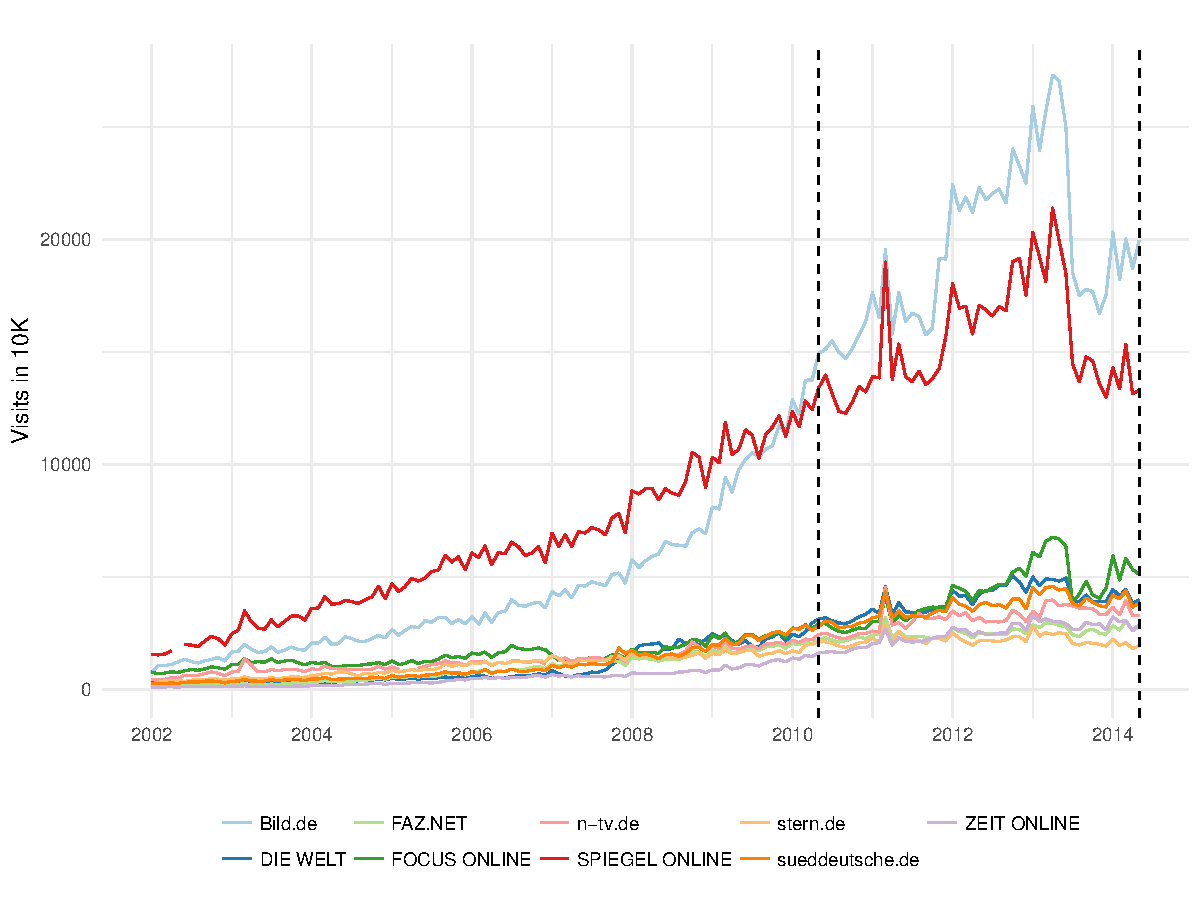
\includegraphics[scale=.6]{../figs/fig_news2}
	\label{}
\end{figure}

\subsection{AR Order: arima(1,0,0)}

\begin{figure}[H]\centering
\caption{Time Series of visits (residuals)}
	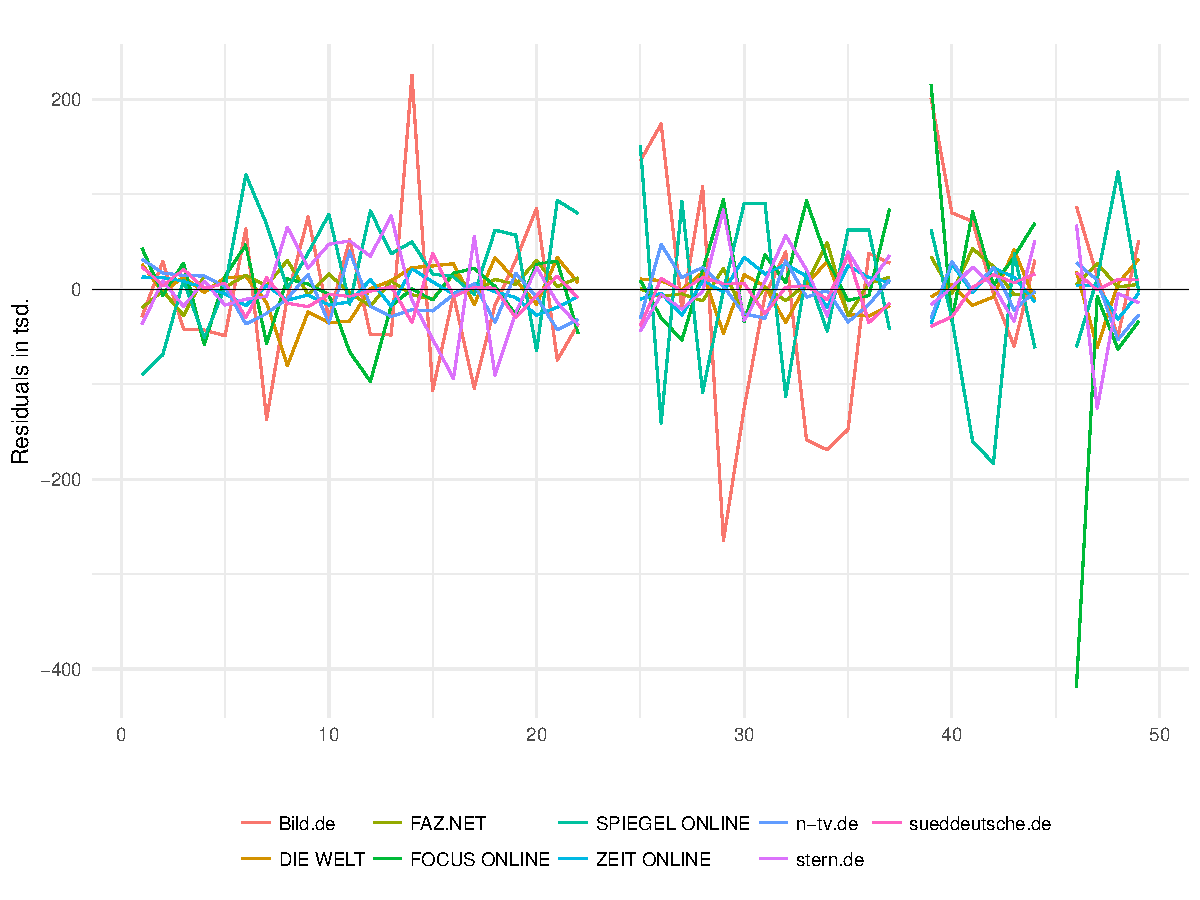
\includegraphics[scale=.6]{../figs/resid_news1}
	\label{}
\end{figure}

\begin{figure}[H]\centering
\caption{Contemporary Crosscorrelation}
	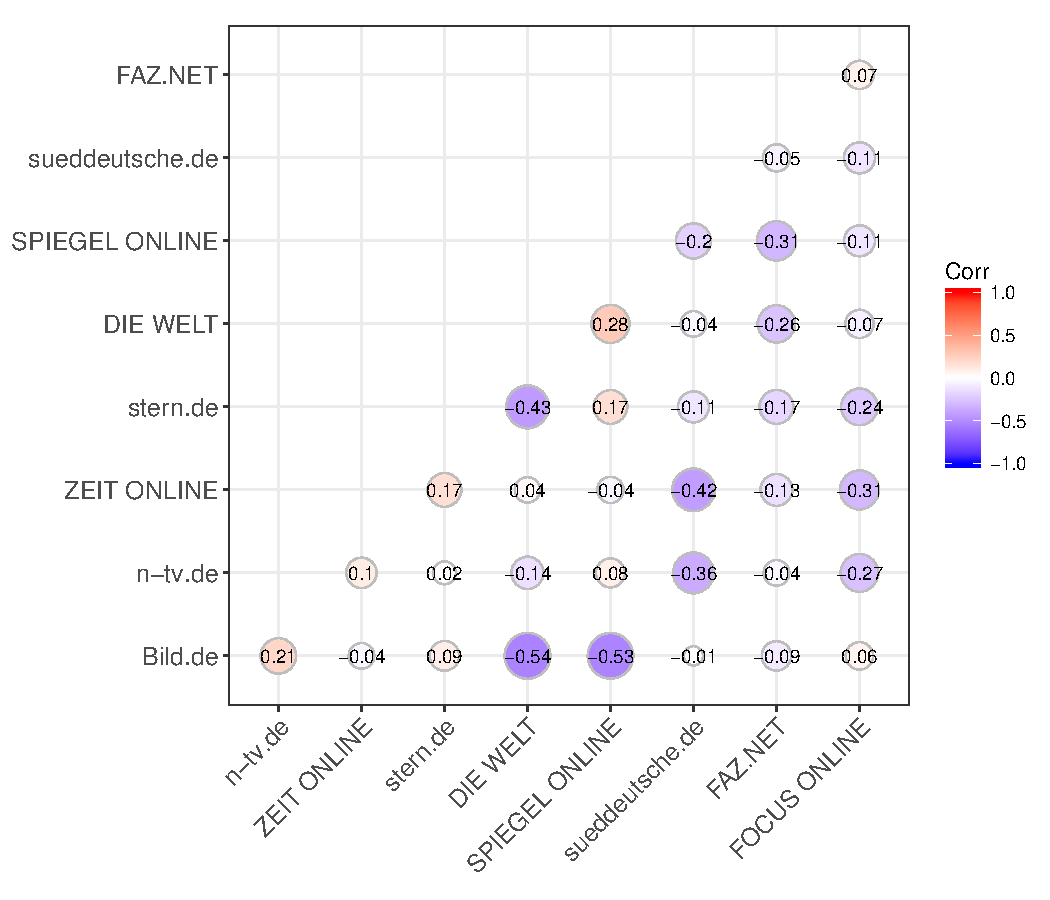
\includegraphics[scale=.7]{../figs/ccf_news}
	\label{}
\end{figure}

\begin{figure}[H]\centering
\caption{Autocorrelation of residuals}
	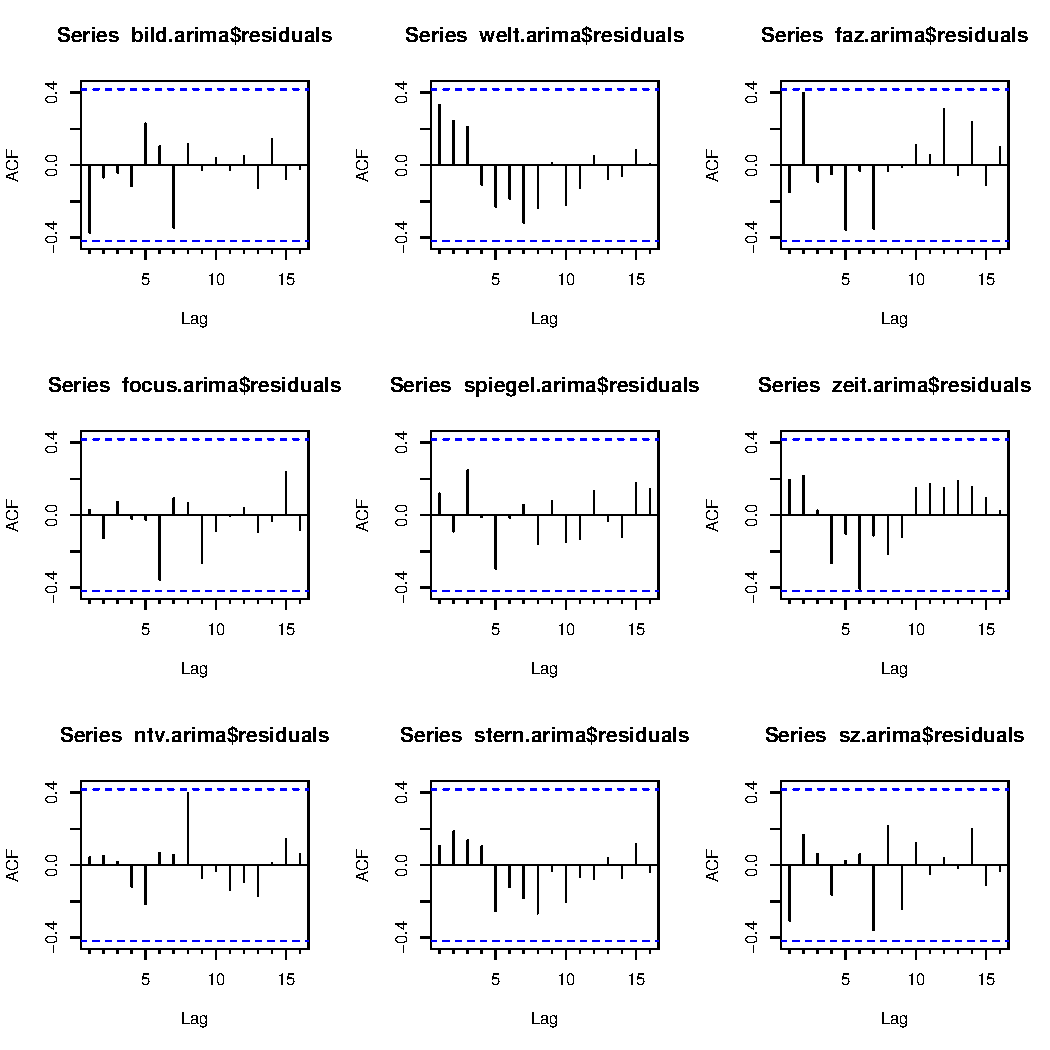
\includegraphics[scale=.7]{../figs/acf_news1}
	\label{}
\end{figure}

\end{document}
